\textbf{Validation and feature ablation.} Validation selected count smoothing $\alpha=3$, logistic inverse regularization $C=0.1$ and rank cap 4. Enlarging the direct classifier's training pool and adding its own selected nodes did not displace the original 64-node MEDUSA+ pool under the validation selection rule. The conditional logistic model's validation edge Brier score was 0.04566. Removing its confidence features raised the score to 0.04795, the largest change among the seven single-group ablations. Removing the uncertainty features raised it to 0.04597. These are conditional edge scores among accepted parents. The path scores in the main comparison apply to whole prefixes.

\textbf{Path calibration.} On 256,000 evaluation candidate nodes, 2.71\% matched the reference continuation. MEDUSA+ had the lowest Brier score (0.01839). Dynamic conditional regression had the lowest binned ECE (0.00125). Conditional counting improved on the fixed marginal model in both Brier and ECE. Small differences in average probability error need not alter which nodes enter the tree.

\begin{figure}[ht]\centering
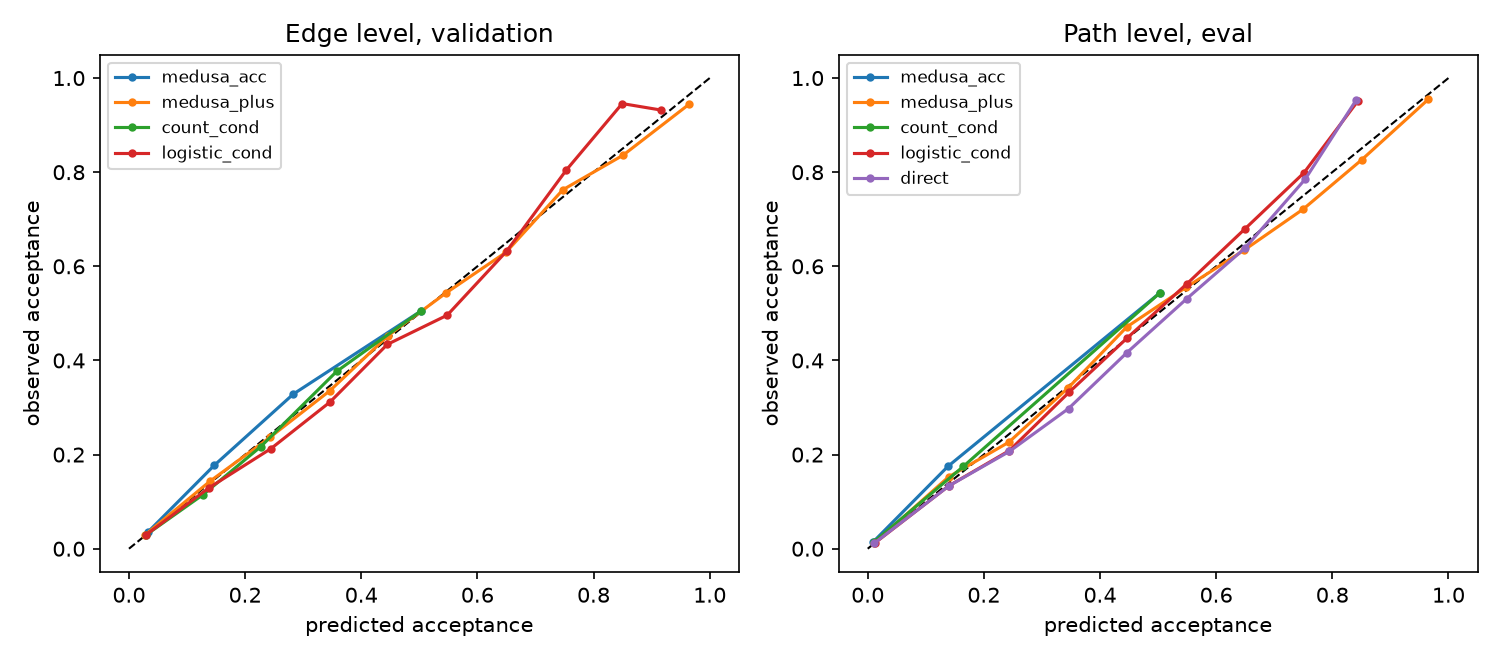
\includegraphics[width=.96\linewidth]{evidence/reliability.png}
\caption{Observed hit rate against predicted probability. The diagonal denotes perfect bin-level agreement. Left: validation child edges evaluated among matching parents. Right: complete candidate paths from a common MEDUSA+ pool on MT-Bench. The panels concern different populations and targets.}
\end{figure}
\begin{table}[ht]\centering
\caption{Validation edge Brier score after refitting with one feature group removed. Positive changes indicate worse prediction. Values are rounded after differencing.}
\begin{tabular}{lrr}\toprule
Omitted group & Brier score & Change from full\\\midrule
None (full model) & .045657 & ---\\
Confidence & .047945 & +.002288\\
Uncertainty & .045974 & +.000317\\
Interactions & .045838 & +.000180\\
Depth & .045721 & +.000064\\
Node rank & .045699 & +.000042\\
Path probability & .045666 & +.000009\\
Parent rank & .045658 & +.000001\\\bottomrule
\end{tabular}
\end{table}

The ablation measures the information each group adds when the other six remain available. A small change after omitting parent rank is compatible with related information surviving in interactions. Likewise, low average path error alone gives little leverage on a budget decision: most paths in the shared pool miss, while the builder compares scores near its frontier.
